\scanpage{26}
\[
u_+\qquad\frac12(u_++u_-)
\]
\[
\underbrace{\left(x+\frac12y\right)}_{\unsure{m|u}}u_+
+\underbrace{\frac12y}_{\unsure{n|v}}u_-
\]

\diagram{\begin{tikzcd}
0\arrow[r]&\unsure{\Pi|\pi}\arrow[r,dash]&V\arrow[r,dash]&E\arrow[r]&0
\end{tikzcd}}

\[
H^1(\unsure{\langle\sigma\rangle|\sigma},E)\xrightarrow{\sim}
\unsure{H^2|H^1}(\sigma,\unsure{\Pi|\pi})\simeq\unsure{\Pi|\pi}^{\sigma}/(1+\sigma)(\unsure{\Pi|\pi})
\]

\[
z\longmapsto\exp 2i\pi z
\]

\figure{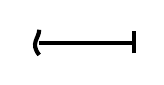
\begin{tikzpicture}[line width=1.5pt]
\draw (0,0)--(1.2,0);\draw (0,-.15)..controls (-.12,0) and (0,.06)..(0,.17);\draw (1.2,-.13)--(1.2,.16);
\end{tikzpicture}}

\figure{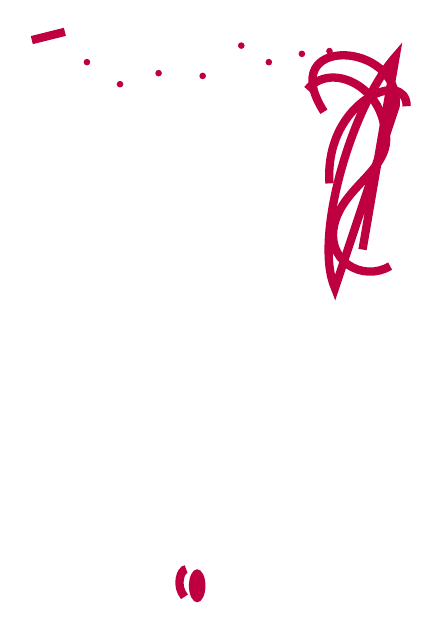
\begin{tikzpicture}[x=.7cm,y=.7cm,line width=3pt,purple]
\draw (0,4)..controls (.4,4.5) and (1.3,4.1)..(1.4,3.3)..controls (1.6,2.6) and (.7,2.3)..(.5,1.6)..controls (.3,.9) and (1,.5)..(1.5,.8);
\draw (.3,3.6)..controls (-.6,5) and (1.7,4.9)..(1.6,3.7)--(.5,.4)..controls (.1,1.3) and (.8,3.7)..(1.6,4.6)--(1,1.1);
\draw (.4,2.3)..controls (.3,3.8) and (1.8,4.4)..(1.8,3.7);
\draw (-5,4.9)--(-4.4,5.05);
\foreach \x/\y in {-4/4.5,-3.4/4.1,-2.7/4.3,-1.9/4.25,-1.2/4.8,-.7/4.5,-.1/4.65,.4/4.7} {\fill (\x,\y) circle (.06);}
\fill (-2,-5) ellipse (.15 and .3);\draw (-2.23,-5.2)..controls (-2.4,-5) and (-2.3,-4.7)..(-2.2,-4.7);
\end{tikzpicture}}
% archive foliation: 28
